\documentclass[11pt, oneside]{article}   	% use "amsart" instead of "article" for AMSLaTeX format
\usepackage{geometry}                		% See geometry.pdf to learn the layout options. There are lots.
\geometry{letterpaper}                   		% ... or a4paper or a5paper or ... 
%\geometry{landscape}                		% Activate for for rotated page geometry
%\usepackage[parfill]{parskip}    		% Activate to begin paragraphs with an empty line rather than an indent
\usepackage{graphicx}				% Use pdf, png, jpg, or eps§ with pdflatex; use eps in DVI mode
								% TeX will automatically convert eps --> pdf in pdflatex		
\usepackage{amssymb}
\usepackage{amsmath}

\usepackage{url}
\usepackage{hyperref}

\title{Notes on continuous- and discrete-time chemical master equation kinetics}
\author{Vincent Voelz}
\date{May 4, 2018}							% Activate to display a given date or no date

\begin{document}
\maketitle


\section*{The Chemical Master Equation}


The \textbf{chemical master equation} describes the time evolution of the populations of multiple chemical species, based on their rates of interconversion:
\[
\frac{d}{dt} \mathbf{p} = \mathbf{K} \mathbf{p}
\]
Here, $\mathbf{p} = (p_1, p_2, ..., p_n)$ is a column vector of state populations (i.e. chemical species), and $\mathbf{K}$ is a \textit{rate matrix}.  The solution of this equation gives the time evolution of the populations $\mathbf{p}(t)$  in terms of the initial populations $\mathbf{p}(0)$, and some properties of the rate matrix $\mathbf{K}$.

\subsection*{A two-state master equation}

As a simple example, let's first consider the case when $n=2$. Here, there are two chemical species, $A$ and $B$, and a reaction $A \rightarrow B$ with forward rate $k_f$ (s$^{-1}$) and backward rate $k_b$ (s$^{-1}$).

\begin{figure}[htbp]
\begin{center}
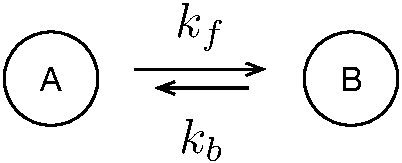
\includegraphics[width=0.3\textwidth]{two-state}
%\caption{\label{fig:your-figure}Caption goes here.}
\end{center}	
\end{figure}

The population flux of the species is described by the differential equations
\[
\frac{d}{dt} p_A = -k_f p_A + k_b p_B 
\]
\[
\frac{d}{dt} p_B = +k_f p_A - k_b p_B
\]
Or, more consisely,
\[
\frac{d}{dt} \begin{pmatrix}
	p_A \\
	p_B \end{pmatrix} = \begin{pmatrix}
	-k_f & k_b \\
	k_f  & -k_b \end{pmatrix} \begin{pmatrix}
	p_A \\
	p_B \end{pmatrix} 
\]
This is now in the form of a master equation with $\mathbf{p} = (p_A, p_B)$ and $\mathbf{K} = \begin{pmatrix}
	-k_f & k_b \\
	k_f  & -k_b \end{pmatrix} $:
\[
\frac{d}{dt} \mathbf{p} = \mathbf{K} \mathbf{p}
\]

Note that the rate matrix $\mathbf{K}$ is \textit{singular} (i.e. \textit{degenerate}), meaning it's not invertible because one row of this matrix is a linear combination of the other.  This means that the determinant of this matrix will be zero, and there must be at least one eigenvalue of $K$ that is zero.

This fact has physical significance.  Consider the eigenvector $\psi$ whose corresponding eigenvalue is zero.  For this eigenvector, 
\[
\frac{d}{dt} \mathbf{p} = \mathbf{K} \psi = 0.
\]
Thus, when the populations are $(p_A, p_B) = \psi$, the dynamics have reached a \textit{steady-state} condition; in other words: $\psi$ are the steady-state populations.

Under the stronger condition where \textit{detailed balance} is obeyed (i.e. $p_A k_f = p_B k_b$, as must be the case for all processes at \textit{equilibrium}), then $\psi = \mathbf{p}_{eq}$ must be the \textit{equilibrium} populations.

\paragraph{Exercise 1.} Use the equilibrium constant $K_{eq} = k_f/k_b$ along with the constraint $p_A + p_B = 1$ to solve for the equilibrium populations $\mathbf{p}_{eq}$.

\paragraph{Exercise 2.} Use the master equation to show that $\mathbf{p}_{eq}$ is the dynamical steady-state. Show that $\mathbf{p}_{eq}$ obeys detailed balance, and therefore are also the equilibrium populations.

\paragraph{Exercise 3.} Find the equilibrium populations $\mathbf{p}_{eq}$ a different way, this time by finding the eigenvalues and eigenvectors of $\mathbf{K}$ ($\mathbf{p}_{eq}$ will be the eigenvector whose corresponding eigenvector is zero).


\subsection*{A many-state master equation}
  
Now consider the case where we have $n$ states, whose populations change according to simple first-order kinetic rates.  We define $k_{ji}$ to be the rate at which species $i$ converts to species $j$.\footnote{NOTE: This nomenclature ($k_{ji}$ used for $k_{i \rightarrow j}$) can be confusing; the reason for this is so  the elements of the rate matrix $K_{ij}$ correspond to row $i$ and column $j$.   Be aware that other authors define the rate matrix using the opposite convention, and then define the master equation in terms of $d\mathbf{p}/dt = \mathbf{pK}$ where $\mathbf{p}$ is a \textit{row} vector.}

The differential equations describing the population flux are:

$$\frac{dp_1}{dt} = -(k_{21}+k_{31}+ ... +k_{n1})p_1 + k_{12} p_2 +k_{13} p_3 + ... +  k_{1n} p_n $$
$$\frac{dp_2}{dt} = k_{21} p_1 + -(k_{12}+k_{32}+ ... +k_{n2})p_2 + k_{23} p_3 + ... +  k_{2n} p_n $$
$$ ... $$
$$\frac{dp_n}{dt} = k_{n1} p_1 + k_{n2} p_2 + ...   -(k_{1n}+k_{2n}+ ... +k_{(n-1)n})p_n$$

This can be expressed succinctly as the master equation  $\frac{d}{dt} \mathbf{p} = \mathbf{K} \mathbf{p}$ where $\mathbf{K}$ is the rate matrix
$$\mathbf{K} =
 \begin{pmatrix}
  -\sum_{i \neq 1} k_{i1} & k_{12} & \cdots & k_{1n} \\
  k_{21} & -\sum_{i \neq 2}k_{i2} & \cdots & k_{2n} \\
  \vdots  & \vdots  & \ddots & \vdots  \\
  k_{n1} & k_{n2} & \cdots & -\sum_{i \neq n}k_{in}
 \end{pmatrix}
$$

\subsection*{Solving the chemical master equation}

Recall that that for a one-dimensional differential equation $dp/dt = \lambda p$, the solution is:
\[
p(t) = p_0 \exp(\lambda t)
\]
where $p_0$ is the initial value of $p$ at time $t=0$.   The strategy for solving the multi-state master equation will be to transform to a new coordinate system in which the rate matrix is diagonal.  In this new (``primed'') coordinate system, the master equation will read
\[
\frac{d}{dt} \mathbf{p}' =  \begin{pmatrix}
  \lambda_1 & 0 & \cdots & 0 \\
 0 & \lambda_2 & \cdots & 0 \\
  \vdots  & \vdots  & \ddots & \vdots  \\
  0 & 0 & \cdots & \lambda_n
 \end{pmatrix} \mathbf{p}' 
\]
This equation describes $n$ independent first-order equations whose solutions are
$$p_i'(t) = p_i'(0) \exp (\lambda_i t)$$
where $i = 1, ... n$.
 
To perform this coordinate transformation, we must find the eigenbasis of $\mathbf{K}$.  Let $\mathbf{V}$ be the matrix whose columns are (right) eigenvectors of $\mathbf{K}$. Then
\[
\mathbf{K} \mathbf{V} = \mathbf{V} \mathbf{\Lambda}
\]
where $\mathbf{\Lambda}$ is the diagonal matrix containing the eigenvalues of $\mathbf{K}$.  Let $\mathbf{p}'(t)$ be the populations in the new coordinate system, such that
$$\mathbf{V}\mathbf{p}' = \mathbf{p}$$
so that the master equation reads:

$$\frac{d}{dt} \mathbf{V}\mathbf{p}' = \mathbf{K} \mathbf{V}\mathbf{p}'$$



Applying $\mathbf{V}^{-1}$ yields
$$\mathbf{V}^{-1} \frac{d}{dt} \mathbf{V}\mathbf{p}' = \mathbf{V}^{-1} \mathbf{K} \mathbf{V}\mathbf{p}'$$
$$\frac{d}{dt} \mathbf{p}'=  \mathbf{\Lambda} \mathbf{p}'$$

We now have $n$ independent first-order equations whose solutions are
$$p_i'(t) = p_i'(0) \exp (\lambda_i t)$$

Transforming back to the original coordinate system (see Appendix for how this works), we get:
$$\mathbf{p}(t) = \sum_{i=1}^n [\psi^L_i \cdot  \mathbf{p}(0)] \psi^R_i \exp (\lambda_i t)$$

where $\psi_i^R$ and $\psi_i^L$ are the right and left eigenvectors (respectively) of $\mathbf{K}$ .  

\subsection*{The time-evolution of state populations is a superposition of relaxation eigenmodes}

In the previous section (and Appendix), we find that the complete solution is the sum
\[
\boxed{
\mathbf{p}(t) = \sum_{i=1}^n [\psi^L_i \cdot  \mathbf{p}(0)] \psi^R_i \exp (\lambda_i t)
}
\]
The interpretation of this solution is a \textbf{superposition of relaxation eigenmodes}. The right eigenvectors of $\mathbf{K}$ give the shape of each eigenmode; the projection of the initial populations onto each \textit{left} eigenvector, $[\psi^L_i \cdot  \mathbf{p}(0)]$, give the \textbf{amplitude} of each relaxation; and the eigenvalues $\lambda_i$ give the \textbf{rate} of each relaxation.

We have already seen in two-state example that one of the eigenvalues of $\mathbf{K}$ is $\lambda_1 = 0$.  It can be proven (not here) that the remaining eigenvalues of  $\mathbf{K}$ are all \textit{less} that zero, and can be ordered 
\[
\lambda_1 > \lambda_2 > ... > \lambda_n.
\]
This means that in the limit of $t \rightarrow \infty$, all the relaxation eigenmodes decay to zero, except for the first eigenmode:
\[
\lim_{t \rightarrow \infty} \mathbf{p}(t) =  [\psi^L_1 \cdot  \mathbf{p}(0)] \psi^R_1 
\]
The first eigenmode $\psi_1^R$ thus proportional to the equilibrium populations, $\mathbf{p}_{eq}$.  In fact, it is typical to define $\psi^R_1 = \mathbf{p}_{eq}$, in which case we also define $\psi^L_1 = (1,1,...,1)$ to maintain the orthogonality of $\psi^L_1$ and $\psi^R_1$. 

What do the other eigenmodes look like?  Let's consider a specific three-state example:


\begin{figure}[htbp]
\begin{center}
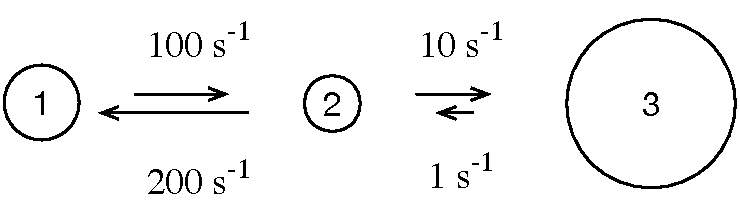
\includegraphics[width=0.6\textwidth]{three-state}
\caption{\label{fig:three-state}A simple three-state kinetic model}
\end{center}
\end{figure}

This model is represented by the following non-zero rates: $k_{21}$ = 100 s$^{-1}$, $k_{12}$ = 200 s$^{-1}$, $k_{32}$ = 10 s$^{-1}$, $k_{23}$ = 1 s$^{-1}$, and a resulting rate matrix of 
\[
\mathbf{K} =
 \begin{pmatrix}
  -\sum_{i \neq 1} k_{i1} & k_{12} & k_{13} \\
  k_{21} & -\sum_{i \neq 2}k_{i2} & k_{23} \\
  k_{31} & k_{32} & -\sum_{i \neq 3}k_{3i}
 \end{pmatrix} =    \begin{pmatrix}
  -100 & 200 & 0 \\
 100 & -210 & 1 \\
  0 & 10 & -1
 \end{pmatrix}\]

Using a numerical eigensolver, we find that the eigenvalues and eigenvectors of this model are
\[
\lambda_1 = 0 \text{ (s}^{-1}),  \lambda_2 = -4.238 \text{ (s}^{-1}),  \lambda_3 = -306.8 \text{ (s}^{-1}),  
\]
There is one \textit{stationary} eigenmode (the equilibirum state), and two \textit{relaxation} eigenmodes that relax on timescales of $\tau_2 = -1/\lambda_2$ = 0.236 s and $\tau_3 = -1/\lambda_3$ = 3.26 ms.

The eigenmodes can be characterized their shape, $\psi_i^R$ and their amplitude $[\psi^L_i \cdot  \mathbf{p}(0)]$.   The eigensolver gives the right eigenvectors as:

\[
\psi_1^R  = \begin{pmatrix} 0.19518  \\ 0.09759 \\ 0.97590 \end{pmatrix}, 
\psi_2^R  = \begin{pmatrix} -0.54104  \\ -0.25906 \\ 0.80010 \end{pmatrix}, 
\psi_3^R  = \begin{pmatrix} -0.69506  \\ 0.71856 \\ -0.02350 \end{pmatrix}, 
\]
But we have some choice in normalizing the left and right eigenvalues so that $(\psi^L_i)^T\psi_j^R = \delta_{ij}$; in particular it's useful normalize the elements of $\psi_1^R$ so it's equal to the equilibrium populations $\mathbf{p}_{eq}$ (making $\psi_1^L = (1,1,1)$. We also have some choice to flip the \textit{sign} of each pair of right and left eigenvalues, so that the amplitude $[\psi^L_i \cdot  \mathbf{p}(0)]$ will always be \textit{positive}.   That way, we can think of each eigenmode $\psi^R_i$ as having an initial positive amplitude, and decaying away over time.  

Let's assume the initial populations at time $t=0$ is given by $\mathbf{p}(0) = (1,0,0)$, i.e. all the population is in state 1. In this case, we inspect the left eigenvectors given by the eigensolver, and flip the sign of both $\psi_i^L$ and $\psi_i^R$ if any of the amplitudes are negative.  We additionally scale the $\psi_i^L$ so that  $(\psi^L_i)^T\psi_j = \delta_{ij}$.

After performing these modifications, we get a new set of eigenmodes and amplitudes:

\[
\psi_1^R  = \begin{pmatrix} 0.1538  \\ 0.0769  \\ 0.7692  \end{pmatrix}, 
\psi_2^R  = \begin{pmatrix} 0.54104  \\ 0.25906 \\ -0.80010 \end{pmatrix}, 
\psi_3^R  = \begin{pmatrix} 0.69506  \\ -0.71856 \\ 0.02350 \end{pmatrix}, 
\]

\[
[\psi^L_1 \cdot  \mathbf{p}(0)] = 1, 
[\psi^L_2 \cdot  \mathbf{p}(0)] = 0.9749, 
[\psi^L_3 \cdot  \mathbf{p}(0)] = 0.4585, 
\]

This information is visually represented in the plot below:

\begin{figure}[htbp]
\begin{center}
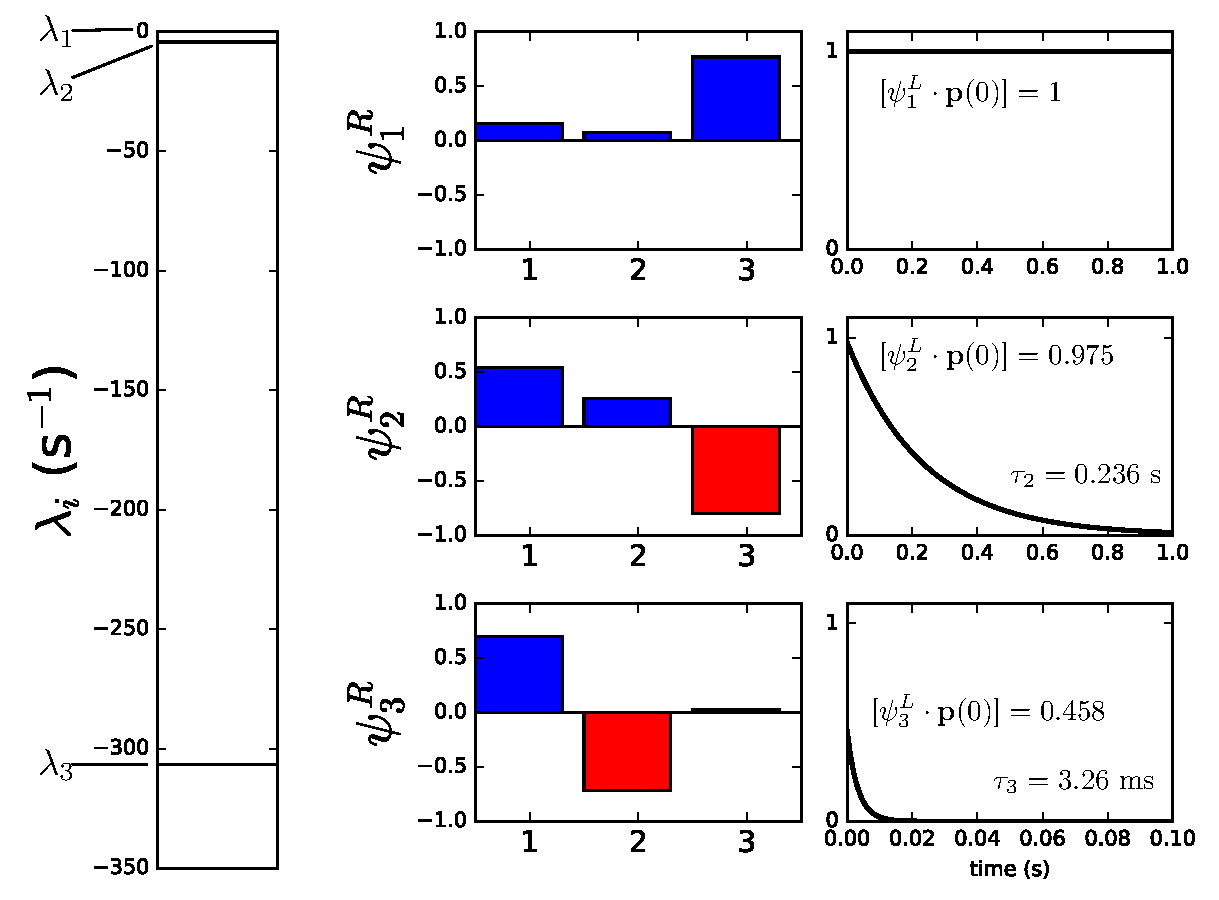
\includegraphics[width=0.8\textwidth]{relaxation-eigenmodes}
\caption{\label{fig:relaxation-eigenmodes}Relaxation eigenmodes of the three-state kinetic model.}
\end{center}
\end{figure}

With this choice of normalization for the left and right eigenvalues, the eigenmodes are more physically meaningful.  The stationary eigenmode, $\psi_1^R  = (0.1538, 0.0769, 0.7692)$, gives the equilibrium populations.  At equilibrium, about 77\% of the population is in state 3.   For the non-stationary modes, the \textit{sign structure} of the eigenmode now shows the \textit{direction} that population is flowing over time, and over what timescale.  For example, from an inspection of the kinetic model in Figure \ref{fig:three-state}, one would predict that if all the population was in state 1 at $t=0$, , there would be a fast \textit{pre-equilibration} between states 1 and 2.  Indeed, the fastest relaxation eigenmode ($\tau_3 \sim 3.26$ ms) is dominated by components 1 and 2. The positive components (blue) show states for which population is leaving on this timescale, and the negative components show states where the population is entering.

\section*{Reconciling experimental and theoretical kinetic models}

\paragraph{Separation of timescales.} A feature evident from Figure \ref{fig:relaxation-eigenmodes} is the clear separation in timescales corresponding to each relaxation eigenmode.  An experiment with limited time-resolution may be able to detect the relaxation on timescale $\tau_2 \sim 0.236$ s, but not the fast relaxation at $\tau_3 \sim 3.26$ ms.   In that case, the experimentalist would conclude a two-state kinetic mechanism, when in reality the situation is more complicated.    This reasoning is often invoked when comparing protein folding experiments to molecular simulations of folding dynamics.  Whereas simulations may identify many microscopic intermediates, experiments may only detect two-state folding behavior.  Figure \ref{fig:ww-eigenmodes} shows the eigenmodes and relaxation time scales for a 200-state kinetic model of WW domain protein folding dynamics. 

\begin{figure}[htbp]
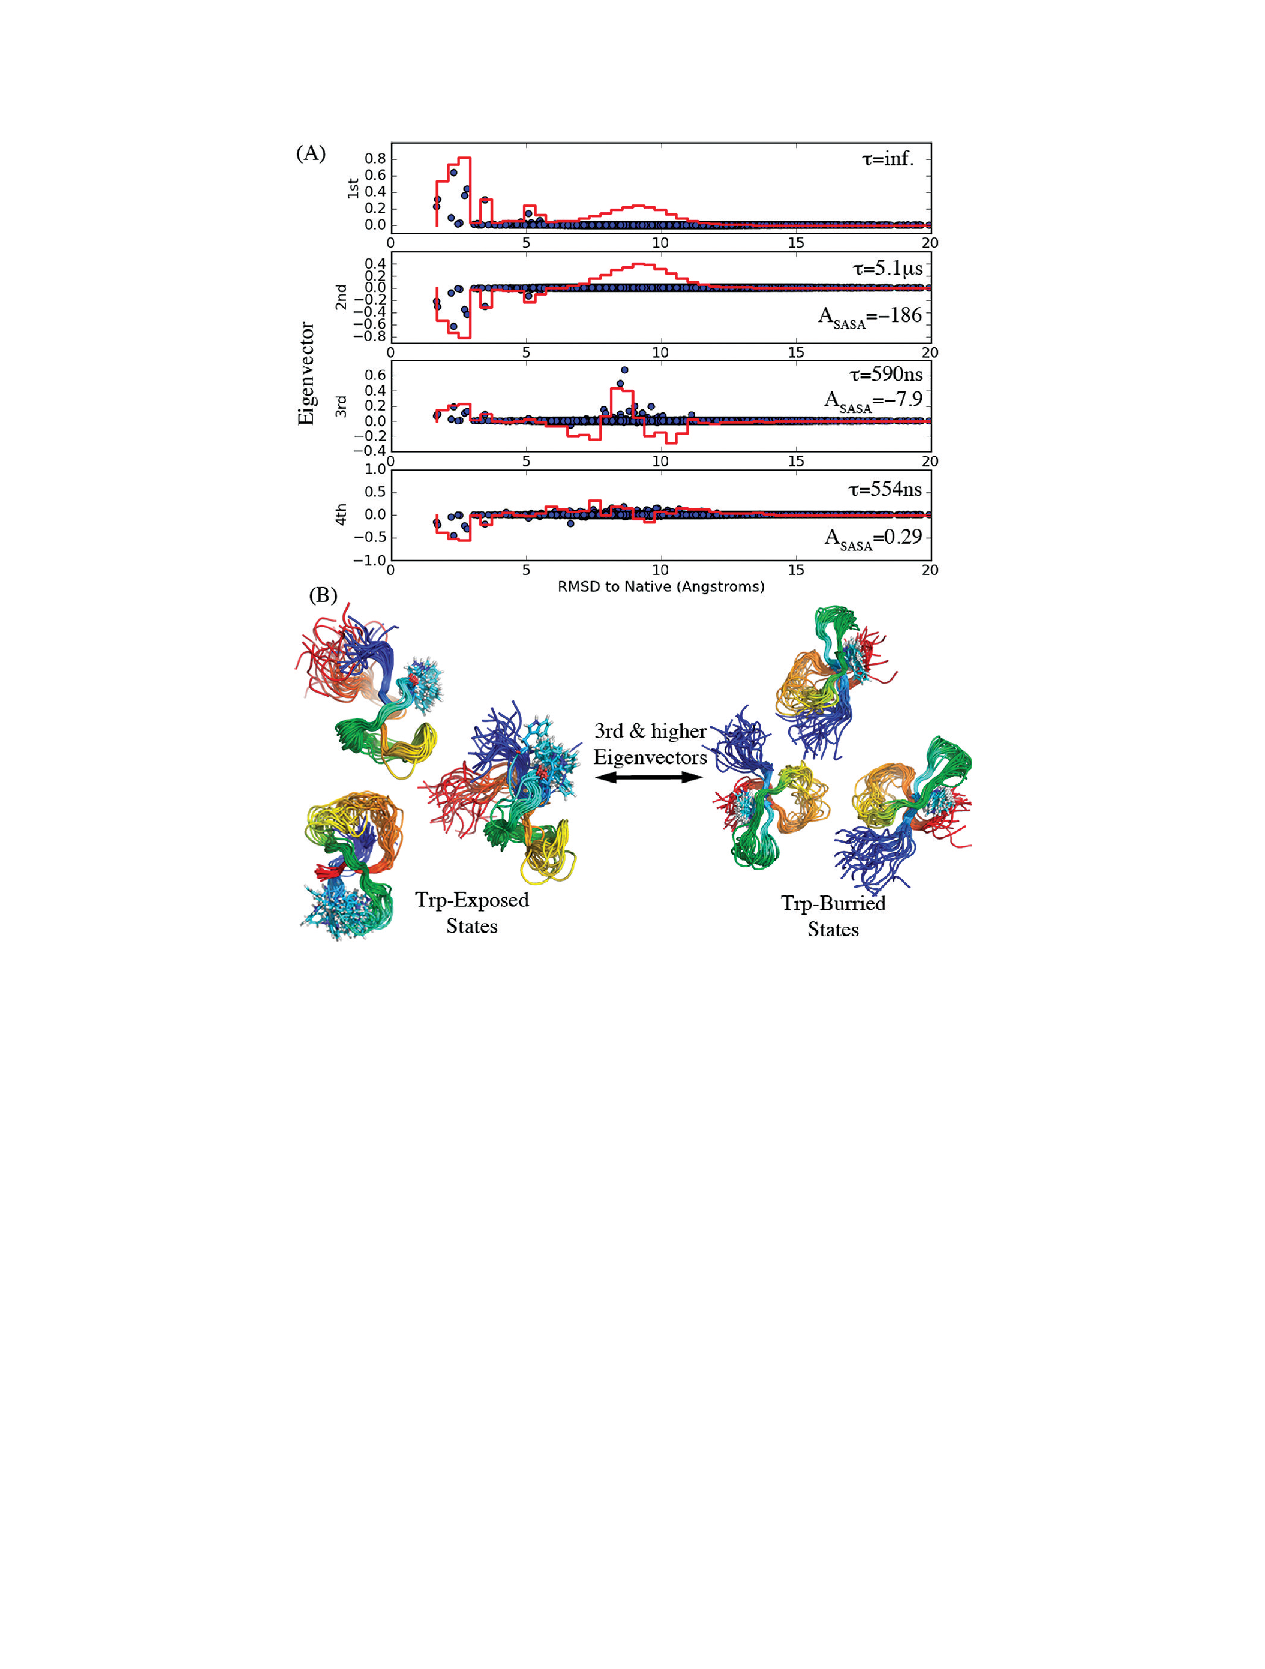
\includegraphics[width=0.8\textwidth]{ww-eigenmodes}
\caption{\label{fig:ww-eigenmodes}A 200-state kinetic model of WW domain protein folding dynamics, constructed from 200 $\mu$s of trajectory data generated on the Anton supercomputer. In order to visualize the relaxation eigenmodes, states are projected to an RMSD-to-native reaction coordinate.  Folding kinetics experiments have shown that  WW domain a two-state folding mechanism, while the simulation-based kinetic model predicts additional fast relaxations ($\sim$ 500 ns) due to the solvent exposure/burial of a tryptophan residue. Figure taken from:  Lane, T. J., et al. (2011). \textit{Journal of the American Chemical Society}, 133(45), 18413--18419. \url{http://doi.org/10.1021/ja207470h} }
\end{figure}

\paragraph{Experimental detection of eigenmode relaxations.} Depending on the situation, there may be problems in experimentally measuring molecular kinetics that give rise the each eigenmode relaxation.  Even if the amplitude $[\psi^L_i \cdot  \mathbf{p}(0)]$ of eigenmode $\psi_i^R$ is significant, it may be that a given spectroscopic observable is very insensitive to population changes captured by $\psi_i^R$.  Consider a vector $\chi$ of experimental observables (e.g. solvent-exposure of a fluorophore) whose elements capture the value of the observable for each of the $n$ kinetic states.  In order to measure relaxation of the $i^{th}$ eigenmode, $\chi \cdot \psi_i^R$ must be sufficiently large to be detected.   

Another case of experimentally ``invisible'' relaxation eigenmodes occurs when the amplitude $[\psi^L_i \cdot  \mathbf{p}(0)]$ of the relaxation is small.   The amplitude depends on the initial (out-of-equilibrium) populations, which can be very different to control exactly.   Protein folding kinetic experiments often use a temperature-jump to perturb the equilibrium populations, so that the relaxation back to equilibrium can be observed.  The initial $\mathbf{0}$ in this case is very similar to $\mathbf{p}_{eq}$, which may result in low amplitudes for some relaxations.  Figure \label{fig:beauchamp} shows a calculation of these amplitudes for eigenmodes of a number of small ``two-state'' proteins.  While many eigenmodes may be present, only a few of them have significant amplitude to be detected experimentally.


\begin{figure}[htbp]
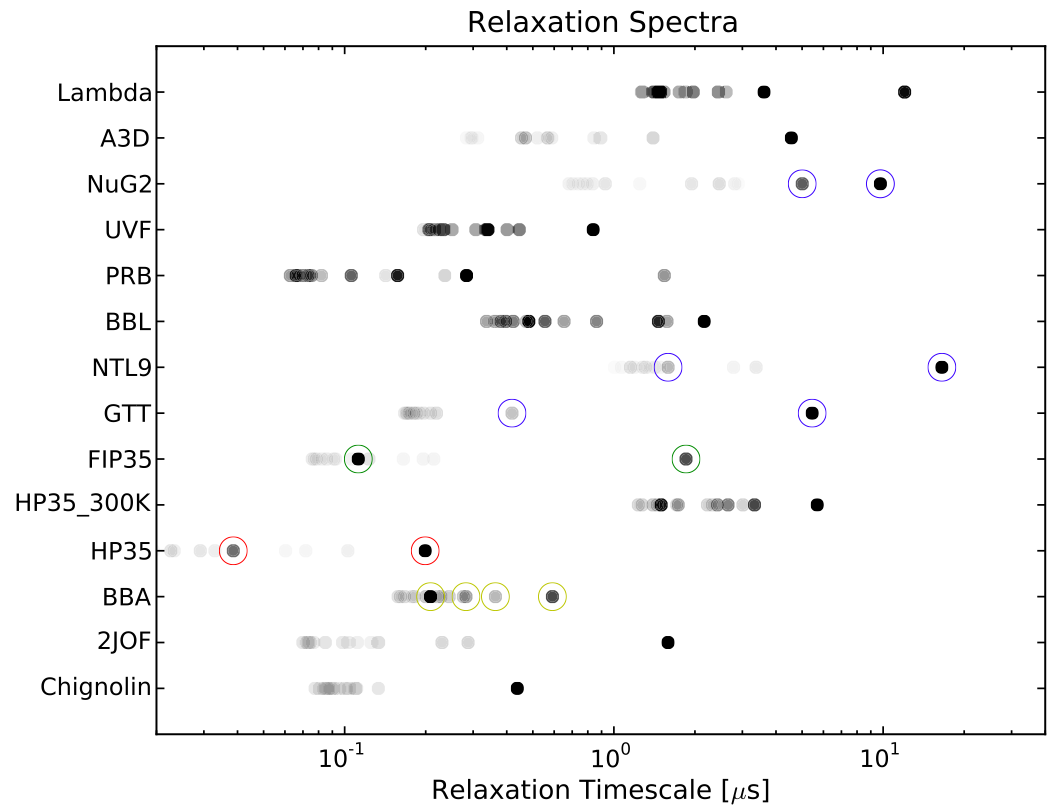
\includegraphics[width=0.8\textwidth]{beauchamp}
\caption{\label{fig:beauchamp} Amplitudes of eigenmodes for a kinetic models of a number of small mini-proteins, constructed from  trajectory data generated on the Anton supercomputer by D. E. Shaw Research.  Figure taken from:  Beauchamp, K. A. et al. (2012). \textit{Proceedings of the National Academy of Sciences of the United States of America}, 109(44), 17807--17813. \url{http://doi.org/10.1073/pnas.1201810109}   }
\end{figure}


\newpage

\subsection*{Discrete-time Markov models}


A Markov model describes population changes in discrete time intervals, using a \textit{transition matrix} $\mathbf{T}^{(\tau)}$, whose elements $T_{ji}$ are probability of transitioning from state $i$ to state $j$ in some time $\tau$.  The time evolution of $\mathbf{p}(t)$ can thus be obtained by iterated multiplication:

$$\mathbf{p}(t+\tau) = \mathbf{T}^{(\tau)}\mathbf{p}(t)$$

From a practical standpoint, transition probabilities $T_{ji}$ are much more easily estimated from molecular simulations than rates. This is because with enough simulation trajectories that start from some state $i$, one can simply \textit{count} how many trajectories have reached state $j$ after some time $\tau$.

\begin{figure}[htbp]
\begin{center}
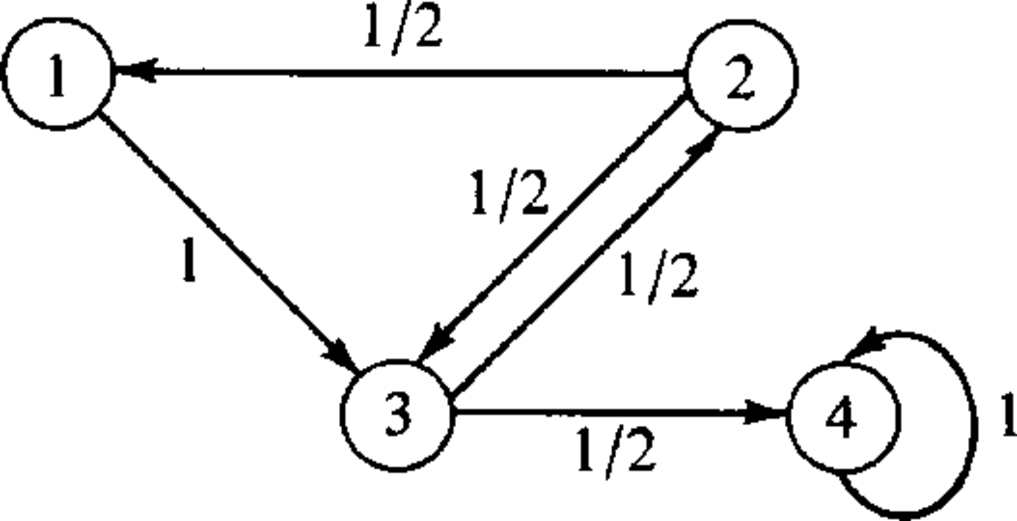
\includegraphics[width=0.4\textwidth]{markov}
\caption{\label{fig:markov}An example of a discrete-time Markov model}
\end{center}
\end{figure}


\subsection*{What is the relationship between $\mathbf{T}^{(\tau)}$ and $\mathbf{K}$?}

Consider the time-evolution of populations according to the master equation $\frac{d}{dt}\mathbf{p}(t) = \mathbf{K} \mathbf{p}$. After some small time interval $\delta t << \tau$ has elapsed, the populations have changed by
$$\delta \mathbf{p} = \mathbf{K}\mathbf{p}(t) \delta t$$
so that 
$$\mathbf{p}(t+\delta t) = \mathbf{p}(t) + \delta \mathbf{p} = (\mathbf{1} + \mathbf{K} \delta t)\mathbf{p}(t)$$


\begin{figure}[htbp]
\begin{center}
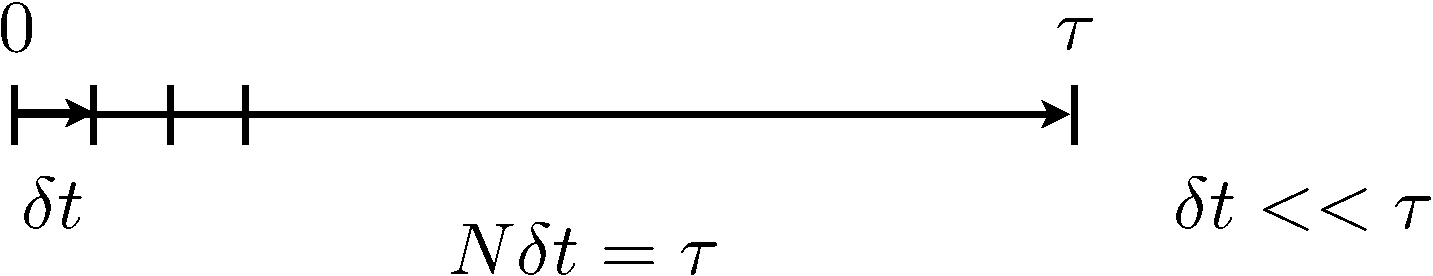
\includegraphics[width=0.6\textwidth]{tau-chopped}
\caption{\label{fig:tau-chopped}}
\end{center}
\end{figure}

If the time window $\tau$ is divided up into $N$  small intervals (such that $N \delta t = \tau$), iteration of the above  yields

$$\mathbf{p}(t+N\delta t) = (\mathbf{1} + \mathbf{K} \delta t)^N\mathbf{p}(t)$$

Taking the limit where $N \rightarrow \infty$ and $\delta t \rightarrow 0$, we get

$$\mathbf{p}(t+\tau) = \lim_{N \rightarrow \infty} (\mathbf{1} + \mathbf{K} \frac{\tau}{N})^N\mathbf{p}(t) = \exp(\mathbf{K}\tau)\mathbf{p}(t)$$

Therefore,
$$\mathbf{T}^{(\tau)} = \exp(\mathbf{K}\tau)$$



\subsection*{$\mathbf{T}^{(\tau)}$ and $\mathbf{K}$ share eigenvectors }

If we write the matrix exponential as an Euler series, we can easily see that $\mathbf{T}^{(\tau)}$ and $\mathbf{K}$ share eigenvectors.  

$$\mathbf{T}^{(\tau)}\psi_i^R = \exp(\mathbf{K}\tau) \psi_i^R$$
$$= [1 + \mathbf{K}\tau + \frac{1}{2!}\mathbf{K}^2\tau^2 + \frac{1}{3!}\mathbf{K}^3\tau^3 + ...] \psi_i^R$$
$$= [1 + \lambda_n\tau + \frac{1}{2!}\lambda_i^2\tau^2 + \frac{1}{3!}\lambda_i^3\tau^3 + ...]  \psi_i^R$$
$$ \mathbf{T}^{(\tau)} \psi_i^R = \exp(\lambda_i \tau) \psi_i^R$$
Apparently, the eigenvalues of $ \mathbf{T}^{(\tau)}$, $\mu_i$, are $\exp(\lambda_i \tau)$.  \textbf{This means we can get information about the timescales of the continuous-time dynamics (i.e. $\lambda_i$) directly through the discrete-time transition matrix}:
$$ \lambda_i = \log(\mu_i)/\tau$$

Useful quantities to define are the so-called \textbf{implied timescales} of each eigenmode relaxation, $\tau_i = -1/\lambda_i$.  We can compute this directly from the discrete-time transition matrix, using

\begin{center}
$\boxed{ \tau_i = \frac{\tau}{-\log(\mu_i)}  }$
\end{center}


\section*{Appendix: Left and Right Eigenvectors}

The eigenvectors $\psi$ referred to in linear algebra are usually \textit{right} eigenvectors:
\[
\mathbf{K} \psi^R = \lambda \psi^R
\]
The \textit{left} eigenvectors are defined by
\[
\psi_i^L \mathbf{K} = \lambda_i \psi_i^L
\]
In the above expression they multiply the matrix as row vectors.   The left and the right eigenvectors are related through the transpose of $\mathbf{K}$, as you can verify in the exercise below:

\paragraph{Exercise.}  Show that the left eigenvectors are the right eigenvectors of $\mathbf{K}^T$ and vice versa.  \textit{Hint:} Take the transpose of both sides of the equation $\mathbf{K} \psi^R = \lambda \psi^R$.  Recall that by the definition of matrix multiplication,  $(\mathbf{ABC})^T = \mathbf{C}^T\mathbf{B}^T\mathbf{A}^T.$ 

\vskip 0.6 cm

Now, consider $\mathbf{V}$ as the matrix whose columns are right eigenvectors $\psi^R_i$ of $\mathbf{K}$.  Since $\mathbf{V}^{-1}\mathbf{KV} = \mathbf{\Lambda}$ is a diagonal matrix, it must be equal to its own transpose:
\[
\mathbf{V}^{-1}\mathbf{KV} = (\mathbf{V}^{-1}\mathbf{KV})^T = \mathbf{V}^T\mathbf{K}^T (\mathbf{V}^{-1})^T
\]
The last term implies that $(\mathbf{V}^{-1})^T$  has the \textit{left} eigenvectors $\psi_i^L$ as its column vectors.  In other words, $\mathbf{V}^{-1}$ is a matrix whose \textit{rows} are the left eigenvectors $\psi_i^L$.   

Since $\mathbf{V}^{-1} \mathbf{V} = \mathbf{1}$, this also means that left and right eigenvectors must obey $\psi_i^L \cdot \psi_j^R = \delta_{ij}$).  Each set of $\psi_i^L$ or $\psi_i^R$ are not in general orthonormal, but through normalization, the products of left and right eigenvector can always be made to equal 1 (when $i=j$) or 0 ($i \neq j$). In the case that the matrix $\mathbf{K}$ is symmetric (i.e. $\mathbf{K}^T = \mathbf{K}$), the left and right are equal to each other, and there is a single set of orthonormal eigenvectors.

\subsection*{Using left and right eigenvectors in the master equation solution}

Recall that in the eigenbasis coordinate system, the solution to the master equation is a column vector $\mathbf{p}'(t)$ whose elements are
\[
p_i'(t) = p_i'(0) \exp (\lambda_i t)
\]
Using $\mathbf{Vp}' = \mathbf{p}$, we can transform back to the original coordinate system:
\[
\mathbf{p}(t) = \mathbf{Vp}'(t) = \sum_i \psi_i^R p_i'(0) \exp (\lambda_i t)
\]
Next, using $\mathbf{p}' = \mathbf{V}^{-1}\mathbf{p}$, we can get $p_i'(0)$ in terms of the original coordinate system.   Since $\mathbf{V}^{-1}$ is a matrix whose rows are the left eigenvectors, $\psi^L_i$, the $i^{th}$ element of $\mathbf{V}^{-1}\mathbf{p}(0)$ is
\[
p_i'(0) = (\psi^L_i)^T\mathbf{p}(0) =  \psi^L_i \cdot \mathbf{p}(0) 
\]
Thus, the complete solution of the master equation is
\[
\mathbf{p}(t) = \sum_i [ \psi^L_i \cdot \mathbf{p}(0)  ] \psi_i^R \exp (\lambda_i t)
\]


\end{document}  